\chapter{Scalability, Performance and Resource Management}\label{ch:perf}

\section{Scalability Requirements}
The system is meant for the load of one transport office or a small state-level pilot:
a few dozen staff and citizens at the same time, not thousands. The requirements we set
were modest and measurable. Typical read operations should return well within a second;
the key look-ups used on every request must not slow down as the tables grow; and a burst
of simultaneous users must produce no errors. Nothing here claims capacity beyond what was
measured.

\section{Workload and Load Model}
The load test uses the most common operation, the \emph{list page}. Six read endpoints
of the backend were requested in rotation: the dashboard summary, and the paged lists of
citizens, vehicles, applications, challans and payments (15 rows per page). Each virtual
user is one thread with its own persistent HTTP connection that issues 60 requests in
turn. The test was run with 1, 5, 10 and 20 concurrent users. A short warm-up preceded the
measurements so that the JVM, the connection pool and the database cache were warm.
Sign-in, which is deliberately slow, was timed separately (ten sign-ins in a row).

\section{Resource Utilisation}
\begin{table}[H]
\centering\small
\caption{Resources observed on the development machine}\label{tab:res}
\begin{tabularx}{\linewidth}{@{}p{5.2cm}X@{}}
\toprule \textbf{Item} & \textbf{Observation}\\ \midrule
Backend process memory & about 110~MB working set (48 threads) while idle after the tests\\
Executable sizes & backend JAR 55.5~MB, portal JAR 20.8~MB\\
Demonstration database & 0.98~MB of data and 2.02~MB of indexes (about 870 rows in 63 tables)\\
Connection pool & at most 20 connections (HikariCP)\\
\bottomrule
\end{tabularx}
\end{table}
The memory figures for the portal and for MySQL read unusually low in the task list (the
operating system trims idle processes), so we do not report them. The data volume is tiny,
which is why Section~\ref{sec:indexres} also tests tables of up to 500\,000 rows.

\section{Concurrent Processing}
The backend handles each request on its own thread and borrows one database connection
for the length of the transaction. Contention appears only where several transactions
want the same row, and then the row locks of Chapter~\ref{ch:algo} make the later ones wait
briefly instead of failing. Reads that do not lock (the lists in this test) run in parallel.

\section{Scheduling and Synchronisation Analysis}
The system does not implement its own CPU scheduler; thread scheduling belongs to the
operating system and the web server. Synchronisation is done by the database: row locks
(\cmd{SELECT ... FOR UPDATE}), guarded updates and unique keys. The concurrency tests in
Section~\ref{sec:conc} check that this synchronisation is correct.

\section{Performance Measurement Method}
The load generator is a short Python program that uses plain HTTP connections. For each
request it records the elapsed time; at the end it reports, per concurrency level, the
number of requests, the number of errors, the elapsed wall-clock time, the throughput, the
average, median and 95th-percentile latency, and the maximum. The test client, the portal,
the backend and the database all ran on the same laptop, so the numbers include the cost of
sharing the processor, and the figures are indicative of this machine, not of a server.

For the index experiment, two synthetic tables with the same columns as the project's
\cd{payment_attempts} and \cd{road_tax_records} were filled with 10\,000, 100\,000 and
500\,000 rows in a scratch database. The same query was timed before and after the
project's indexes were created, and \texttt{EXPLAIN} recorded the plan. The median of
repeated runs is reported.

\section{Performance Results}
\subsection{Load test}\label{sec:loadres}
Table~\ref{tab:load} gives the results. There were \textbf{no failed requests at any
level} (2\,160 requests in total).

\begin{table}[H]
\centering\small
\caption{Concurrent-user results (read operations, one machine)}\label{tab:load}
\begin{tabularx}{\linewidth}{@{}cccccccc@{}}
\toprule \textbf{Users} & \textbf{Requests} & \textbf{Errors} & \textbf{Time (s)} & \textbf{Throughput (req/s)} & \textbf{Mean (ms)} & \textbf{p95 (ms)} & \textbf{Max (ms)}\\ \midrule
1 & 60 & 0 & 1.36 & 44.2 & 22.6 & 49.9 & 72.7\\
5 & 300 & 0 & 1.62 & 185.5 & 26.6 & 55.9 & 142.2\\
10 & 600 & 0 & 1.81 & 331.3 & 28.5 & 62.0 & 132.4\\
20 & 1\,200 & 0 & 3.16 & 380.3 & 46.2 & 158.0 & 590.9\\
\bottomrule
\end{tabularx}
\end{table}

\begin{figure}[H]
\centering
\begin{subfigure}{0.48\linewidth}
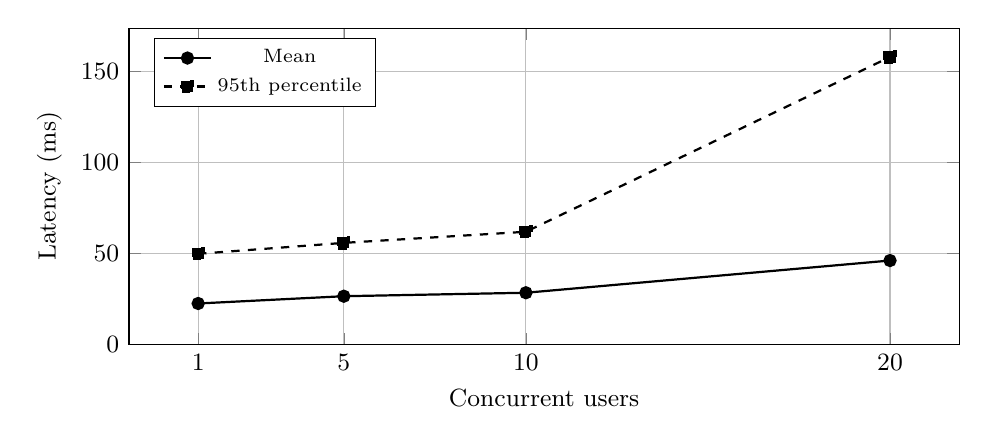
\begin{tikzpicture}
\begin{axis}[width=\linewidth,height=5.6cm,xlabel={Concurrent users},ylabel={Latency (ms)},xtick={1,5,10,20},ymin=0,
  legend style={font=\scriptsize,at={(0.03,0.97)},anchor=north west},grid=major,tick label style={font=\small},label style={font=\small}]
\addplot[mark=*,thick] coordinates {(1,22.6)(5,26.6)(10,28.5)(20,46.2)};
\addplot[mark=square*,thick,dashed] coordinates {(1,49.9)(5,55.9)(10,62.0)(20,158.0)};
\legend{Mean,95th percentile}
\end{axis}
\end{tikzpicture}
\caption{Latency}
\end{subfigure}\hfill
\begin{subfigure}{0.48\linewidth}
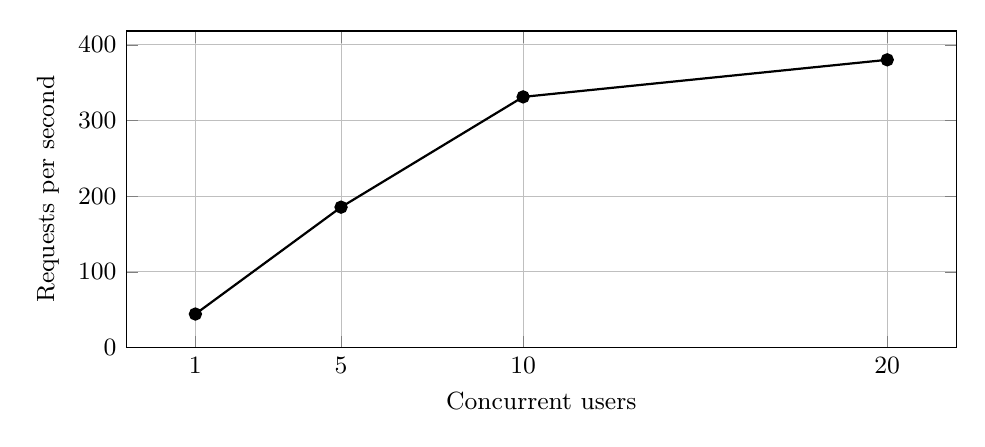
\begin{tikzpicture}
\begin{axis}[width=\linewidth,height=5.6cm,xlabel={Concurrent users},ylabel={Requests per second},xtick={1,5,10,20},ymin=0,
  grid=major,tick label style={font=\small},label style={font=\small}]
\addplot[mark=*,thick] coordinates {(1,44.2)(5,185.5)(10,331.3)(20,380.3)};
\end{axis}
\end{tikzpicture}
\caption{Throughput}
\end{subfigure}
\caption{Load-test results for one to twenty concurrent users}\label{fig:loadplot}
\end{figure}

\paragraph{Reading the results.} Mean latency rose only from 22.6~ms to 46.2~ms while the
load grew twenty-fold, and throughput rose from 44 to 380 requests per second. The gain
flattens between 10 and 20 users (331 to 380 requests per second) while the 95th
percentile jumps from 62~ms to 158~ms. That pattern is typical of a machine approaching
saturation: the twelve logical processors were shared among the test client, two Java
processes and MySQL.

\subsection{Individual endpoints and sign-in}
\begin{table}[H]
\centering\small
\caption{Single-user latency per endpoint (30 requests each)}\label{tab:endpoints}
\begin{tabularx}{\linewidth}{@{}Xcc@{}}
\toprule \textbf{Endpoint} & \textbf{Mean (ms)} & \textbf{p95 (ms)}\\ \midrule
Dashboard summary & 21.5 & 24.6\\
Citizens, page of 15 & 12.4 & 18.7\\
Vehicles, page of 15 & 33.4 & 37.4\\
Applications, page of 15 & 10.3 & 12.7\\
Challans, page of 15 & 9.9 & 11.8\\
Payments, page of 15 & 21.8 & 28.0\\
\bottomrule
\end{tabularx}
\end{table}
Sign-in averaged \textbf{445~ms} (maximum 483~ms) over ten consecutive attempts. This is
not a defect. BCrypt at cost 12 is \emph{meant} to be slow, because that slowness is what
protects stored passwords against guessing \cite{provos1999,owasp-pw}.

\subsection{Effect of the indexes}\label{sec:indexres}
Table~\ref{tab:index} and Figure~\ref{fig:indexplot} show the index experiment.

\begin{table}[H]
\centering\small
\caption{Query time with and without the project's index (median of repeated runs)}\label{tab:index}
\begin{tabularx}{\linewidth}{@{}rCCCC@{}}
\toprule
\textbf{Rows} & \multicolumn{2}{c}{\textbf{Payment-attempt lookup by gateway reference}} & \multicolumn{2}{c}{\textbf{Overdue road-tax count (status, due date)}}\\
 & Without (ms) & With (ms) & Without (ms) & With (ms)\\ \midrule
10\,000 & 4.28 & 0.67 & 6.84 & 0.96\\
100\,000 & 76.71 & 0.81 & 53.34 & 2.64\\
500\,000 & 405.88 & 1.38 & 266.49 & 14.32\\
\bottomrule
\end{tabularx}
\end{table}

\begin{figure}[H]
\centering
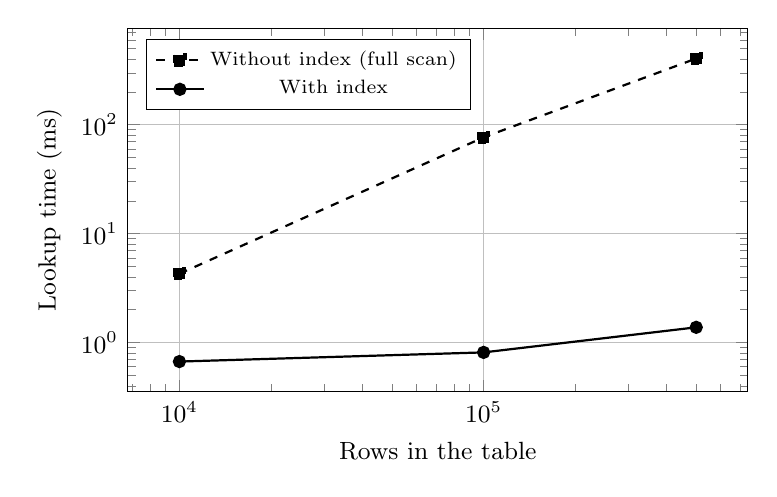
\begin{tikzpicture}
\begin{loglogaxis}[width=0.78\linewidth,height=6.2cm,xlabel={Rows in the table},ylabel={Lookup time (ms)},grid=major,
  legend style={font=\scriptsize,at={(0.03,0.97)},anchor=north west},tick label style={font=\small},label style={font=\small}]
\addplot[mark=square*,thick,dashed] coordinates {(10000,4.283)(100000,76.706)(500000,405.882)};
\addplot[mark=*,thick] coordinates {(10000,0.669)(100000,0.812)(500000,1.38)};
\legend{Without index (full scan),With index}
\end{loglogaxis}
\end{tikzpicture}
\caption{Gateway-reference lookup time against table size (both axes logarithmic)}\label{fig:indexplot}
\end{figure}

\begin{table}[H]
\centering\small
\caption{Query plans at 500\,000 rows (from \texttt{EXPLAIN})}\label{tab:explain}
\begin{tabularx}{\linewidth}{@{}p{3.5cm}p{2.6cm}p{3.6cm}p{2.3cm}X@{}}
\toprule \textbf{Query} & \textbf{Access type} & \textbf{Key used} & \textbf{Rows examined} & \textbf{Extra}\\ \midrule
Lookup, no index & ALL & none & 498\,454 & Using where\\
Lookup, with index & ref & idx\_attempt\_gateway\_ref & 1 & --\\
Road-tax count, no index & ALL & none & 498\,834 & Using where\\
Road-tax count, with index & range & idx\_road\_tax\_status\_due & 28\,742 & Using where; Using index\\
\bottomrule
\end{tabularx}
\end{table}
At 500\,000 rows the indexed lookup was about 290 times faster. The scan time grows with
the table size (4.3, 76.7 and 405.9~ms) while the indexed lookup stays between 0.7 and 1.4~ms,
which matches the $O(n)$ against $O(\log n)$ analysis of Chapter~\ref{ch:algo}. The
road-tax query gains less (about 19 times) because it returns a count over a range of about
29\,000 matching entries, which is work the index cannot avoid; it still reads only the index
(\texttt{Using index}) and not the table.

\section{Bottleneck Identification}
\begin{itemize}
\item \textbf{Sign-in} is the slowest operation by design (about 0.45~s).
\item \textbf{Full scans} are the main data-related risk. Without the indexes, a lookup on 500\,000 rows takes about 0.4~s, and it would be paid on every payment request.
\item \textbf{Shared machine.} At 20 users the 95th percentile rose to 158~ms; part of that is the load generator competing with the servers.
\item \textbf{Vehicle list.} The vehicle list was the slowest endpoint (33~ms); it joins several reference tables to show names. Its time is acceptable but it is the first place to look if lists slow down.
\end{itemize}

\section{Optimisation and Improvement}
The indexes of Table~\ref{tab:indexes} are the main optimisation, and the experiment above
confirms their effect. Other measures already in place are paging (at most 100 rows), a
connection pool, queries that select only what a page shows, and keeping permission
look-ups to two short queries. Further options are listed in Section~\ref{sec:opt}. We
did not make any other change merely because it seemed faster; each would have to be
justified by a measurement like these.

\section{Deployment and Resource Use}
The system runs as two executable JAR files and a MySQL service on one machine
(Figure~\ref{fig:deploy}). Nothing in the build is specific to a cloud provider. The
single-process design means a hosting service that runs Java 21 and offers MySQL would be
enough for a pilot; no such deployment was tried and none is claimed.

\section{Scalability Limitations}
\begin{itemize}
\item The tests used one machine and read-only list requests. Write-heavy and mixed workloads were exercised for correctness (Section~\ref{sec:conc}) but not timed at scale.
\item The revoked-token set is in memory, so it would need a shared store before several backend instances could be run.
\item Offset paging gets slower for very deep pages on very large tables.
\item The tested table sizes (up to 500\,000 rows) are far below those of a national register.
\item The portal keeps a session per user in the memory of its single process.
\end{itemize}
